\section{Лекция 12}

\textbf{Теор.} Если $u(x) \in W^2_{\infty} (\Omega)$, то $ \exists v \in H_N$:
\[ {\|u-v\|}_{L_{\infty}(\Omega)} \leq c_3 h^2 {\|u\|}_{W^2_{\infty}(\Omega)}\]
\[ \| u-v \|_{W_{\infty}^1} \leq c_4 h \|u\|_{W^2_{\infty}(\Omega)}\]

Если $u \in C^2(\Omega)$, то
\[ {\|u-v\|}_{C(\Omega)} \leq c_5 h^2 {\|u\|}_{C^2(\Omega)} \]

\textbf{Упр.} Доказать теорему.
\[ \varphi_i(x) = \frac{1}{\sqrt{h}}
\left\{
\begin{array}{ll}
	\cfrac{x-x_{i-1}}{h_i}, \qquad & x \in (x_{i-1}, x_i) \\
	\cfrac{x_{i+1} - x}{h_{i+1}}, \qquad & x \in (x_i, x_{i+1}) \\
	0, \qquad & x \in (x_{i-1}, x_{i+1})
\end{array}
\right. \qquad i = \overline{1, N-1}
\]
\[ v(x) = \Sum_{i=0}^{N} \sqrt{h} u(x_i) \varphi_i(x) \]

\textbf{Пример}
\[
\left\{
\begin{array}{l}
	- \cfrac{d}{dx} \left(p(x) \cfrac{du}{dx} \right) + q(x) u = f(x), \qquad p(x) >0, \quad q(x) \geq 0, \quad f \in L_2(a, b) \\
	u(a) = \cfrac{du}{dx}(b) = 0
\end{array}
\right.
\]
\[ H_A: \quad {\|u\|}_A = \sqrt{\Int_{a}^{b} \left(p \, {\left|\frac{du}{dx}\right|}^2+q {\left| u \right|}^2 \right) dx} \]
\[ H_N = L (\varphi_0, ..., \varphi_N) \]

\subsection{Билинейные базисные функции в $\mathbb{R}^2$}

Пусть $\Omega$ --- некоторая прямоугольная область в $\mathbb{R}^2$
\[ A_0 = x_0 < x_1 < ... < x_{N_x} < A_1, \qquad \Delta x_i = x_i - x_{i-1}, \quad \Delta x = \underset{i=1, N_x}{\max} \Delta x_i \]
\[ B_0 = y_0 < y_1 < ... < y_{N_y} = B_1, \qquad \Delta y_1 = y_i - y_{i-1}, \quad \Delta y = \underset{i=1, N_y}{\max} \Delta y_i \]
\[ h = \max \ (\Delta x, \Delta y) \]
\[ \varphi_i(x) =
\left\{
\begin{array}{ll}
	\cfrac{x_i - x_{i-1}}{\Delta x_i}, \qquad & x \in (x_{i-1}, x_i) \\
	\cfrac{x_{i+1} - x}{\Delta x_{i+1}}, \qquad & x \in (x_i, x_{i+1}) \\
	0, \qquad & x \not \in (x_{i-1}, x_{i+1})
\end{array}
\right.
\]
\[ \varphi_j(y) =
\left\{
\begin{array}{ll}
	\cfrac{y_j - y_{j-1}}{\Delta y_j}, \qquad & y \in (y_{j-1}, y_j) \\
	\cfrac{y_{j+1} - y}{\Delta y_{j+1}}, \qquad & y \in (y_j, y_{j+1}) \\
	0, \qquad & y \not \in (y_{j-1}, y_{j+1})
\end{array}
\right.
\]
\[ Q_{ij} (x, y) = \varphi_i(x) \varphi_j(y) \]
\[ u^h(x,y) = \Sum_{i, j} a_{ij} Q_{ij}(x, y), \qquad (x_i, y_j) \in \overline{\Omega} \]
\[ L(Q_{ij}) = W_2^{1, h} \cap W_2^1 \] \\

\textbf{Теор.} Если $ u \in C^{(2)} (\Omega)$, то существует  $u^h \in W^{1, h}_2$ такая, что
\[ {\|u - u^h\|}_{L_2(\Omega)} \leq c h^2 {\|u\|}_{C^{(2)} (\Omega)} \]
\[ {\|u-u^h\|}_{W_2^1(\Omega)} \leq c h {\| u \|}_{C^{(2)} (\Omega)} \]

где $c = const$ не зависит от $h, u$ \\

\underline{Док-во}
\[ u^h(x,y) = \Sum_{i, j} u(x_i, y_j) Q_{ij}(x, y) \]
\[ \xi (x, y) = u(x, y) - u^h(x,y) \]
\begin{multline*}
	\xi(x, y) = (x - x_l) \frac{\partial \xi}{\partial x} (x_l, y_k) + (y - y_k) \frac{\partial \xi}{\partial y} (x_k, y_k) + \Int_{x_l}^{x} dx' \Int_{x_l}^{x'} \frac{\partial^2 \xi}{{\partial x''}^2} (x'', y_k) dx'' + \\
	+ \Int_{y_k}^{y}dy' \Int_{y_k}^{y'} \frac{\partial ^2 \xi}{{\partial y''}^2}(x_l, y'') d y'' + \underbrace{\Int_{x_l}^{x} \Int_{y_k}^{y} \frac{\partial ^2 \xi}{\partial x' \partial y'} (x', y') dx' dy'}_{C}
\end{multline*}

\[\frac{\partial^2 u^h}{\partial x \partial y} = \frac{1}{\Delta x_{l+1} \Delta y_{k+1}} \Int_{x_l}^{x_{l+1}} dx' \Int_{y_k}^{y_{k+1}} \frac{\partial^2 u}{\partial x' \partial y'}(x', y') \, dy',\]


\[\raisebox{.5pt}{\textcircled{\raisebox{-.9pt} {A}}} \quad (x - x_l) \frac{\partial \xi}{\partial x}(x_l, y_k) = \frac{x - x_l}{\Delta x_{l+1}}
\Int_{x_l}^{x_{l+1}} dx' \Int_{x'}^{x_l} \frac{\partial^2 u}{{\partial x''}^2}(x'', y_k) \, dx'',\]
\[\raisebox{.5pt}{\textcircled{\raisebox{-1.5pt} {B}}} \quad \Int_{x_l}^x dx' \Int_{x_l}^{x'} \frac{\partial^2 \xi}{{\partial x''}^2}(x'', y_k) dx'' = 
\Int_{x_l}^x dx' \Int_{x_l}^{x'} \frac{\partial^2 u}{{\partial x''}^2}(x'', y_k) \, dx'',\]
\begin{multline*}
	\raisebox{.5pt}{\textcircled{\raisebox{-1.5pt} {C}}}
	\quad \Int_{x_l}^x dx' \Int_{y_k}^y \frac{\partial^2 \xi}{\partial x' \partial y'}(x', y') \, dy' = \\
	= \frac{1}{\Delta x_{l+1} \Delta y_{k+1}} \Int_{x_l}^{x_{l+1}} dx'' \Int_{y_k}^{y_{k+1}} dy'' \Int_{x_l}^x dx' \Int_{y_k}^{y'} \left( \frac{\partial^2 u}{\partial x' \partial y'}(x', y') - \frac{\partial^2 u}{\partial x'' \partial y''}(x'', y'') \right) \, dy'
\end{multline*}

Следовательно выражение для $\xi (x,y)$ принимает вид
\begin{multline*}
	\xi(x, y) = \frac{x - x_l}{\Delta x_{l+1}} \Int_{x_l}^{x_{l+1}} dx' \Int_{x'}^{x_l} \frac{\partial^2 u}{{\partial x''}^2}(x'', y_k) \, dx'' + \frac{y - y_k}{\Delta y_{k+1}} \Int_{y_k}^{y_{k+1}} dy' \Int_{y'}^{y_k} \frac{\partial^2 u}{{\partial y''}^2}(x_l, y'') \, dy'' + \\
	+ \Int_{x_l}^x dx' \Int_{x_l}^{x'} \frac{\partial^2 u}{{\partial x''}^2}(x'', y_k) \, dx'' + \Int_{y_k}^y dy' \Int_{y_k}^{y'} \frac{\partial^2 u}{{\partial y''}^2}(x_l, y'') \, dy'' + \\ 
	+ \frac{1}{\Delta x_{l+1} \Delta y_{k+1}} \Int_{x_l}^{x_{l+1}} dx'' \Int_{y_k}^{y_{k+1}} dy'' \Int_{x_l}^x dx' \left( \frac{\partial^2 u}{\partial x' \partial y'}(x', y') - \frac{\partial^2 u}{\partial x'' \partial y''}(x'', y'') \right) dy'
\end{multline*}

Отсюда следует, что
\[ | \xi (x,y) | \leq c \left( {\Delta x_{l+1}}^2 + {\Delta y_{k+1}}^2 \right) \Sum_{|i|=2} {\left\| D^{|i|} u \right\|}_{C(\Omega_{l+1, k+1})} \leq c \left( {\Delta x}^2 + {\Delta y}^2 \right) \Sum_{i=2} {\left\| D^{(i)} u \right\|}_{C(\Omega)} \]
\[ {\| u - u^h \|}_{L_2(\Omega)} = \Int_{\Omega} {| u - u^h |}^2 dx dy \leq c {\left( {\Delta x}^2 + {\Delta y}^2 \right)}^2 {\left( \Sum_{i=2} {\left\| D^{(i)} u \right\|}_{C(\Omega)} \right)}^2 \]

\textbf{Упр.} Получить вторую оценку

\textbf{Упр*.} Доказать более сильную оценку:
\[ {\|u - u^h\|}_{C(\Omega)} \leq c ({\Delta x}^2 + {\Delta y}^2) \Sum_{i=2}^{} {\left\| D^{(i)} u \right\|}_{C (\Omega)}\]

\begin{figure}[h!]
	\begin{center}
		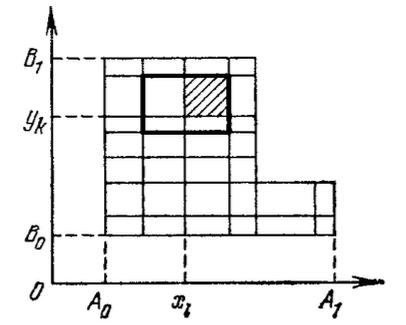
\includegraphics[scale=0.4]{images/12.png}
	\end{center}
	\label{12}
	\caption{Область $\Omega$}
\end{figure}

\[ \left\{
\begin{array}{l}
	- \Delta u + u = f, \qquad f \in L_2 (\Omega) \\
	u|_{\partial \Omega} = g
\end{array}
\right. \]
\[ F(u) = \Int_{\Omega} \left( {\left( \frac{\partial u}{\partial x} \right)}^2 + {\left( \frac{\partial u}{\partial y} \right)}^2 + u^2 - 2uf \right) dx dy \]
\[ H_A = \accentset{\circ}{W}_2^1 (\Omega) \]
\[ \accentset{\circ}{W}_2^{1,h} = \left\{ u^h: u^h \in W_2^{1,h}, \quad u^h = \Sum_{i,j} a_{ij} Q_{ij}, \quad {\| u^h \|}_{\accentset{\circ}{W}_2^{1,h}} = {\| u^h \|}_{W_2^{1,h}}, \quad (x_i, y_j) \in \Omega \right\} \]

\textbf{Теор.} Для любой $u \in W_2^1 (\Omega) \cap C^{(2)}(\Omega)$ существует $u^h \in W_2^{1, h}$ такая, что справедливы оценки \eqref{label}.

\subsection{Построение проекционно сеточной схемы для ОДУ 2-го порядка}

Рассмотрим следующую задачу
\[ \left\{
\begin{array}{ll}
	-\cfrac{d}{dx} \left( p(x) \cfrac{du}{dx} \right) + q(x)u(x) = f(x), \qquad & f \in L_2(a, b) \\
	u(a) = u(b) = 0 \qquad & 0< p_0 \leq p(x) \leq p_1,\ 0 \leq q(x) \leq q_1 \\
\end{array}
\right. \]
\[ Au = f \]
\[ H = L_2 (a, b) \ \Rightarrow \ A \ \text{положительно определен} \ \Rightarrow \ \exists A^{-1} \ \Rightarrow \ \exists! \ \text{решение} \ \eqref{label} \]

Пусть $u(x)$ --- решение \eqref{label}
\[ {\|u\|}_{W_2^2 (\Omega)} \leq c \, {\|f\|}_H \]
\[ H_A = \accentset{\circ}{W}_2^1 (\Omega), \qquad c_0 {\|u\|}_{W_2^1} \leq {\| u \|}_A \leq c_1 {\|u\|}_{W_2^1} \]
\[ F(u) = [u, u] -2 (u, f) \rightarrow \min \quad \text{на} \ \accentset{\circ}{W}_2^1 (\Omega)\]
\[ \varphi_i(x) = \frac{1}{\sqrt{h}} \Biggl\{ ... \]
\[ \accentset{\circ}{W}_2^{1, h} = \left\{ v = \Sum_{i=1}^{N-1} a_i \varphi_i (x) \right\} \subset \accentset{\circ}{W}_2^1 = H_A \]
\[ u^h(x) = \Sum_{i=1}^{N-1} a_i \varphi_i (x) \ \text{--- минимизирует} \ F(v) \ \text{на} \ \accentset{\circ}{W}_2^{1, h} \]

Находим $a_j$ из $\cfrac{\partial F}{\partial a} (u_h) = 0, \quad i=\overline{1, N-1}$

Приходим к системе уравнений
\[ \widehat{A} a = f, \qquad \hat{A} = (A_{ij})\]
\[ A_{ij} = [\varphi_i, \varphi_j] = \Int_{\Omega_{ij}}^{} \left( p \frac{d\varphi_i}{dx}\frac{d \varphi_j}{dx} + q \varphi_i \varphi_j \right) dx \]
\[ a = {(a_1, ... , a_{N-1})}^T, \qquad {f = (f_1, ... , f_{N-1})}^T \]
\[ f_i = \Int_{\Omega_i} f \varphi_i dx \]

Существует единственное решение $ {(a_1, ..., a_{N-1})}^T $, которое однозначно определяет решение $ u^h \leftarrow \underset{v \in \accentset{\circ}{W}_2^{1, h}}{\operatorname{argmin}} \ F(v) $

Отметим, что так как $A_{ij} = 0$ при $|i - j|>1$, то матрица $\widehat{A}$ оказывается трехдиагональной. \\

\textbf{Упр.} Найти $ A_{ij}$ в случае кусочно-постоянных $p$ и $q$ на сетке
\[ p_{i-\frac{1}{2}} = p(x), \quad x \in (x_{i-1}, x_i), \qquad i = \overline{1, N} \]
\[ q_{i-\frac{1}{2}} = ... \]

\newpage